\documentclass[a4paper,10pt,ngerman]{scrartcl}
\usepackage{babel}
\usepackage[T1]{fontenc}
\usepackage[utf8x]{inputenc}
\usepackage[a4paper,margin=2.5cm,footskip=0.5cm]{geometry}

% Die nächsten drei Felder bitte anpassen:
\newcommand{\Aufgabe}{Aufgabe 1: \LaTeX-Dokument} % Aufgabennummer und Aufgabennamen angeben
\newcommand{\TeamID}{00000}       % Team-ID aus dem PMS angeben
\newcommand{\TeamName}{Name} % Team-Namen angeben
\newcommand{\Namen}{Vor- und Nachnamen} % Namen der Bearbeiter/-innen dieser Aufgabe angeben
 
% Kopf- und Fußzeilen
\usepackage{scrlayer-scrpage, lastpage}
\setkomafont{pageheadfoot}{\large\textrm}
\lohead{\Aufgabe}
\rohead{Team-ID: \TeamID}
\cfoot*{\thepage{}/\pageref{LastPage}}

% Position des Titels
\usepackage{titling}
\setlength{\droptitle}{-1.0cm}

% Für mathematische Befehle und Symbole
\usepackage{amsmath}
\usepackage{amssymb}

% Für Bilder
\usepackage{graphicx}

% Für Algorithmen
\usepackage{algpseudocode}

% Für Quelltext
\usepackage{listings}
\usepackage{color}
\definecolor{mygreen}{rgb}{0,0.6,0}
\definecolor{mygray}{rgb}{0.5,0.5,0.5}
\definecolor{mymauve}{rgb}{0.58,0,0.82}
\lstset{
  keywordstyle=\color{blue},commentstyle=\color{mygreen},
  stringstyle=\color{mymauve},rulecolor=\color{black},
  basicstyle=\footnotesize\ttfamily,numberstyle=\tiny\color{mygray},
  captionpos=b, % sets the caption-position to bottom
  keepspaces=true, % keeps spaces in text
  numbers=left, numbersep=5pt, showspaces=false,showstringspaces=true,
  showtabs=false, stepnumber=2, tabsize=2, title=\lstname
}
\lstdefinelanguage{JavaScript}{ % JavaScript ist als einzige Sprache noch nicht vordefiniert
  keywords={break, case, catch, continue, debugger, default, delete, do, else, finally, for, function, if, in, instanceof, new, return, switch, this, throw, try, typeof, var, void, while, with},
  morecomment=[l]{//},
  morecomment=[s]{/*}{*/},
  morestring=[b]',
  morestring=[b]",
  sensitive=true
}

% Diese beiden Pakete müssen zuletzt geladen werden
%\usepackage{hyperref} % Anklickbare Links im Dokument
\usepackage{cleveref}

% Daten für die Titelseite
\title{\textbf{\Huge\Aufgabe}}
\author{\LARGE Team-ID: \LARGE \TeamID \\\\
	    \LARGE Team-Name: \LARGE \TeamName \\\\
	    \LARGE Bearbeiter/-innen dieser Aufgabe: \\ 
	    \LARGE \Namen\\\\}
\date{\LARGE\today}

\begin{document}

\maketitle
\tableofcontents

\vspace{0.5cm}

\noindent\textbf{Anleitung:} Trage oben in den Zeilen 8 bis 11 die Aufgabennummer, 
die Team-ID, den Team-Namen und alle Bearbeiter/-innen dieser Aufgabe mit Vor- und Nachnamen ein.
Vergiss nicht, auch den Aufgabennamen anzupassen (statt "`\LaTeX-Dokument"')!\\
   
\noindent Dann kannst du dieses Dokument mit deiner \LaTeX-Umgebung übersetzen.\\

\noindent Die Texte, die hier bereits stehen, geben ein paar Hinweise zur
Einsendung. Du solltest sie aber in deiner Einsendung wieder entfernen!

\section{Lösungsidee}
Die Idee der Lösung sollte hieraus vollkommen ersichtlich werden, ohne dass auf die eigentliche Implementierung Bezug genommen wird.

Der Text wird am besten mit Unterüberschriften strukturiert:
\subsection{Unterüberschrift}
\subsubsection{Unter-Unterüberschrift}
\paragraph{Benannter Absatz} Lorem ipsum.


\subsection{Mathematik}

\begin{align}
 a_0 & := 2 + 3 \\
   & = 3^2 - 2^2
\end{align}

\begin{align}\label{eq:toll}
 \sum_{i=0}^3 i = \prod_{i=1}^3 i = \frac{12}{2} = \sqrt[3]{216}
\end{align}

\begin{align*}
 f(x) \propto  x^2 \Leftrightarrow \exists r \in \mathbb R : \forall x: f(x) = r * x^2 \Rightarrow x \in \mathcal{O}(x^2)
\end{align*}

Mathematische Formeln erhalten normalerweise eine Nummer, die man referenzieren kann.
In \cref{eq:toll} zum Beispiel ist jeder Term gleich $6$.
Mathematische Formeln können auch im Fließtext gesetzt werden: $\sum_{i=0}^3 i = \prod_{i=1}^3 i = \frac{12}{2} = \sqrt[3]{216}.$

\subsection{Algorithmen}
\begin{algorithmic}
\If{$i\geq i_\text{max}$}
  \State $a\gets -1$
\ElsIf{$i\leq i_\text{min}$}
  \State $a\gets 1$
\Else
  \State $a\gets 0$
\EndIf
\For{$i$ from 1 to 10}
  \State $a\gets a + i$
\EndFor
\ForAll{$i$ in $Liste$}
  \State $a\gets a + i$
\EndFor
\While{$a > 0$}
  \State $a\gets a - 1$
\EndWhile
\Repeat
  \State $a\gets a - 1$
\Until{$a < 0$}
\Loop
  \State $i\gets$\Call{Increment}{$i$}
\EndLoop
\Function{Increment}{$a$}
  \State $a \gets a+1$
  \State \Return $a$
\EndFunction
\end{algorithmic}

\subsection{Bilder}

Bilder werden von \LaTeX nicht direkt da angezeigt, wo sie eingebunden wurden, sondern an passenden Stellen in der Nähe.
Das ist so beabsichtigt.
Man kann aber Bilder referenzieren.
Auf \cref{abb:bild1} sieht man irgendwas mit Informatik, auf \cref{abb:bild2} auch.

\begin{figure}
	\begin{center}
		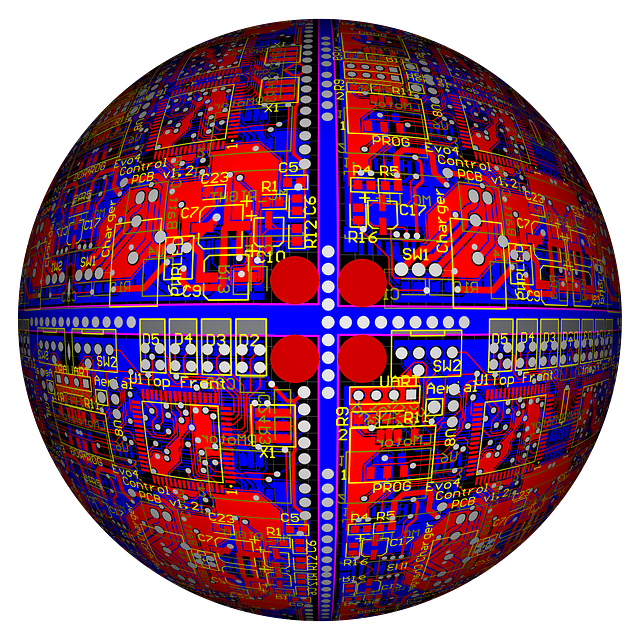
\includegraphics[width=0.3\textwidth]{computerbild1.png}
		\caption{Ein Bild mit irgendwas mit Informatik (Lizenz: CC0)}
		\label{abb:bild1}
	\end{center}
\end{figure}

\begin{figure}
	\begin{center}
		
\includegraphics[width=0.4\textwidth]{computerbild2.jpg}
		\caption{Ein anderes Bild mit irgendwas mit Informatik (Lizenz: CC0)}
		\label{abb:bild2}
	\end{center}
\end{figure}

Man kann Bilder fest positionieren, dann können sie aber keine Bildunterschrift haben und man kann sie nicht referenzieren. Zum Beispiel diese Veranschaulichung einer Queue (Warteschlange):
\begin{center}
	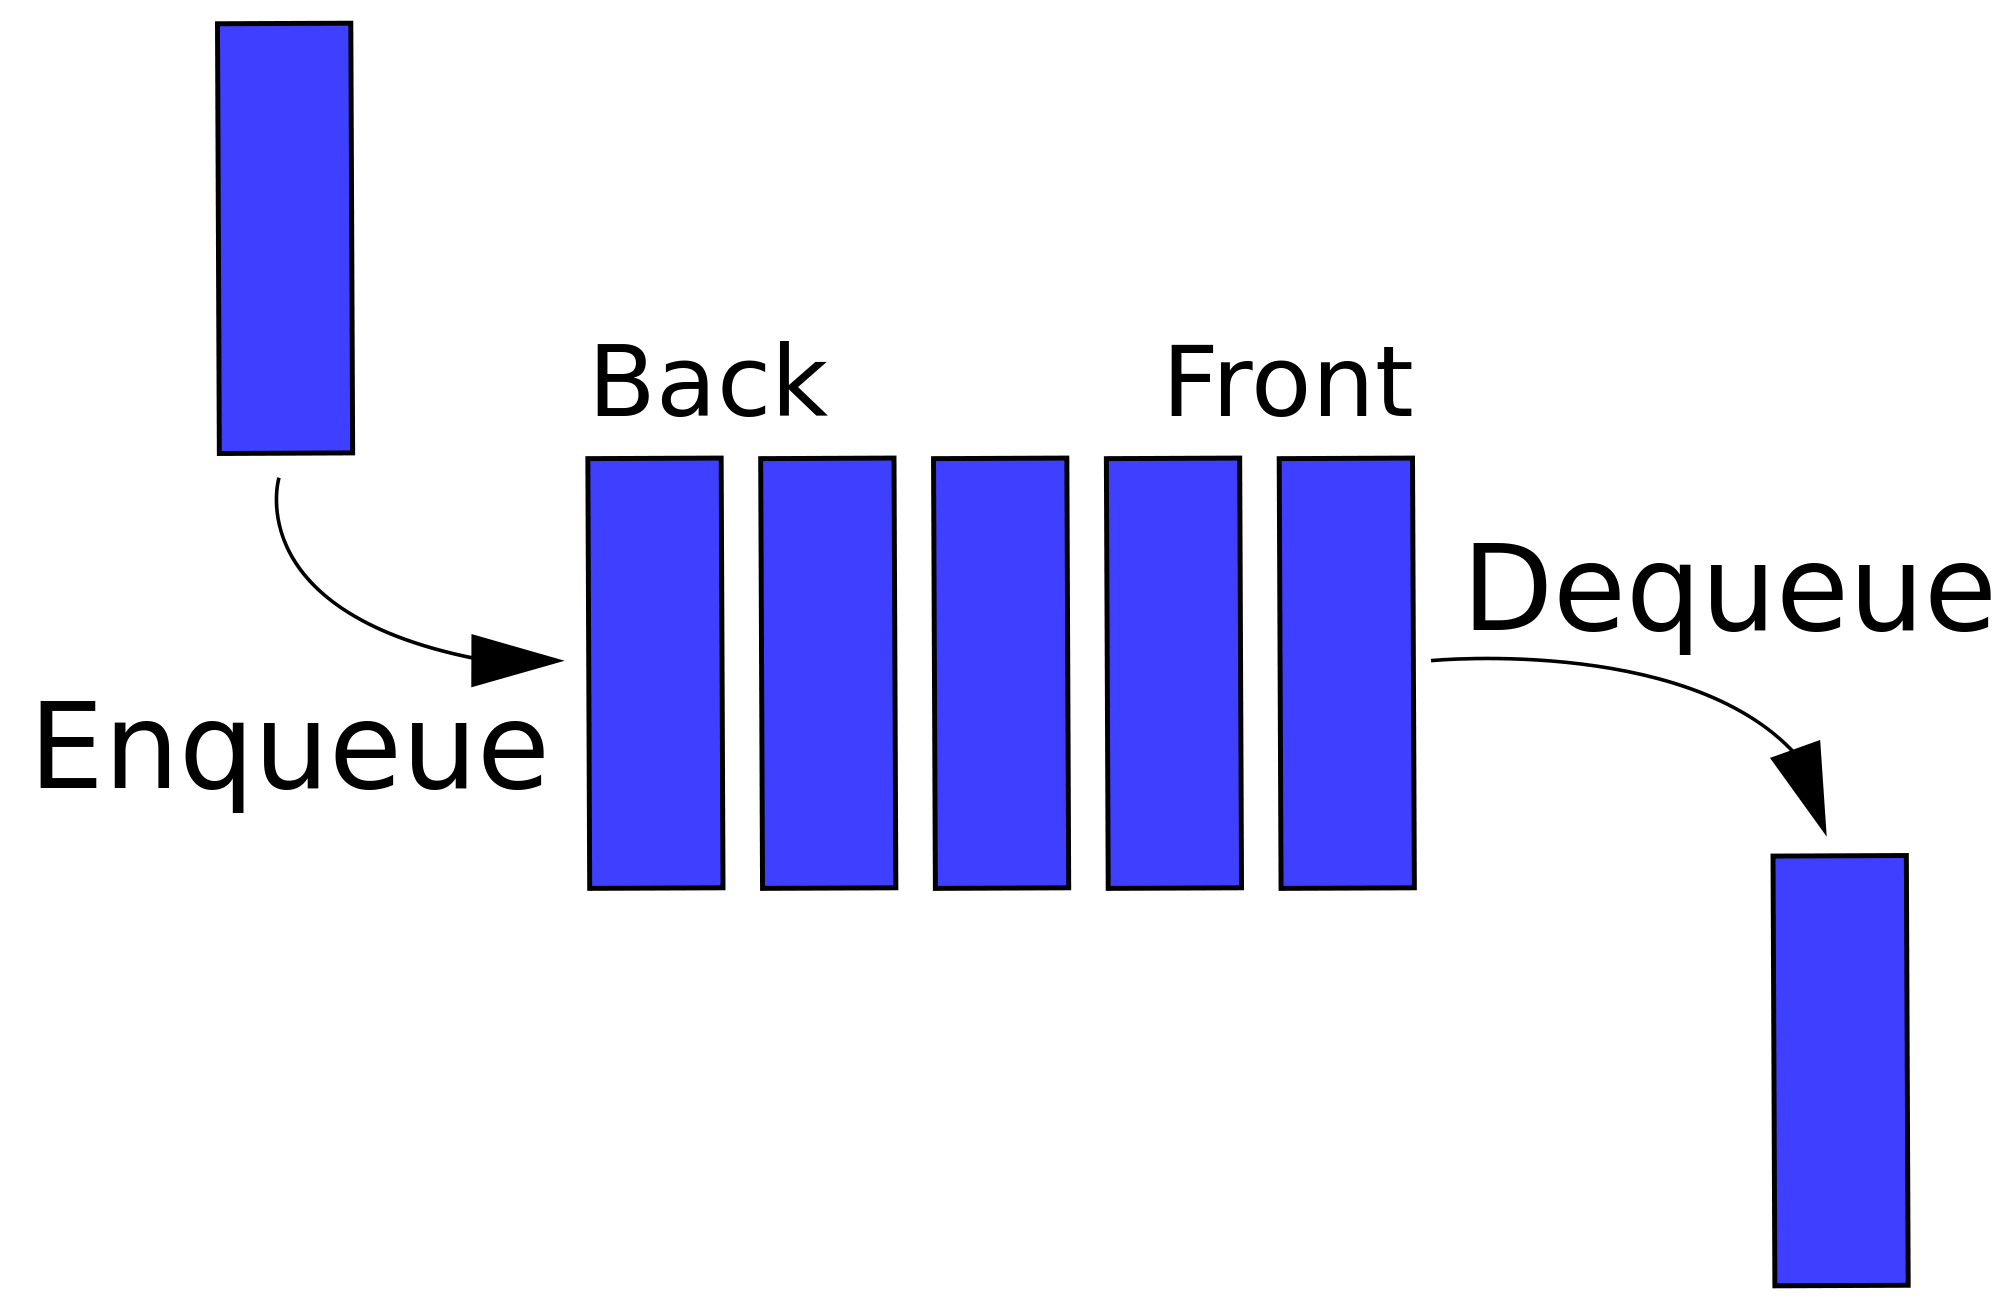
\includegraphics[width=0.4\textwidth]{queue.png}
\end{center}

\section{Umsetzung}
Hier wird kurz erläutert, wie die Lösungsidee im Programm tatsächlich umgesetzt wurde. Hier können auch Implementierungsdetails erwähnt werden.

\section{Beispiele}
Genügend Beispiele einbinden! Die Beispiele von der BwInf-Webseite sollten hier diskutiert werden, aber auch eigene Beispiele sind sehr gut – besonders wenn sie Spezialfälle abdecken. Aber bitte nicht 30 Seiten Programmausgabe hier einfügen!

\section{Quellcode}
Unwichtige Teile des Programms sollen hier nicht abgedruckt werden. Dieser Teil sollte nicht mehr als 2–3 Seiten umfassen, maximal 10.

\lstset{language=Pascal}          % Set your language (you can change the language for each code-block optionally)

\begin{lstlisting}[frame=single,language=Python,title=Kleines Python-Programm]
for i in range(100):
if i % 2 == 0:
pass
else:
print(i)
\end{lstlisting}

\begin{lstlisting}[frame=single,language=C++,title=Kleines C++-Programm]
#include <iostream>

int main(int argc, char** argv) {
std::cout << "Hallo";
return 0;
}
\end{lstlisting}

Hier noch ein kurzes Pascal-Snippet ohne Rahmen:
\begin{lstlisting}[language=Pascal]
for i := maxint to 0 do
begin
a := a + i
end;
Write('Case insensitive ');
Write('Pascal keywords.');
\end{lstlisting}

Das folgende Programm wird aus einer Datei geladen:
\lstinputlisting[frame=single,language=JavaScript,title=Großes JS-Programm]{source.js}

\end{document}
